\documentclass[xcolor={dvipsnames},aspectratio=169,10pt]{beamer}
\usetheme{mx}
\usepackage{graphicx}
\graphicspath{{figures/}}
%\input{preamble.tex}

\title{  
Towards a Simple Framework of Skill Transfer Learning for \\ Robotic Ultrasound-guidance Procedures
}
\subtitle{Robot-Assisted Medical Imaging (RAMI) workshop at ICRA 2023}

\author{
Tsz Yan Leung and
{\bf Miguel Xochicale, PhD} [\faTwitter @\_mxochicale  \faGithub @mxochicale] \\
Research Engineer, advancing AI tools for MedTech and SurgTech 
}
\date{
29th of May 2023
%\today
}
\institute{
Advanced Research Computing Centre and WEISS \\
University College London
}

\githubrepository{https://github.com/mxochicale/rami-icra2023}


\begin{document}

\maketitle


%%%%%%%%%%%%%%%%%%%%%%%%%%%%%%%%%%%%%%%%%%%%%%%%%%%%%%%%
{
\paper{
Leung T. Y. and Xochicale M. in RAMI-ICRA2023 \faGithub \hspace{0em} \url{https://github.com/mxochicale/rami-icra2023}
}

\begin{frame}{
Towards a Simple Framework of Skill Transfer Learning for \\
Robotic Ultrasound-guidance Procedures
}{
Tsz Yan Leung and Miguel Xochicale in RAMI-ICRA2023
}

      \begin{figure}
        \centering
        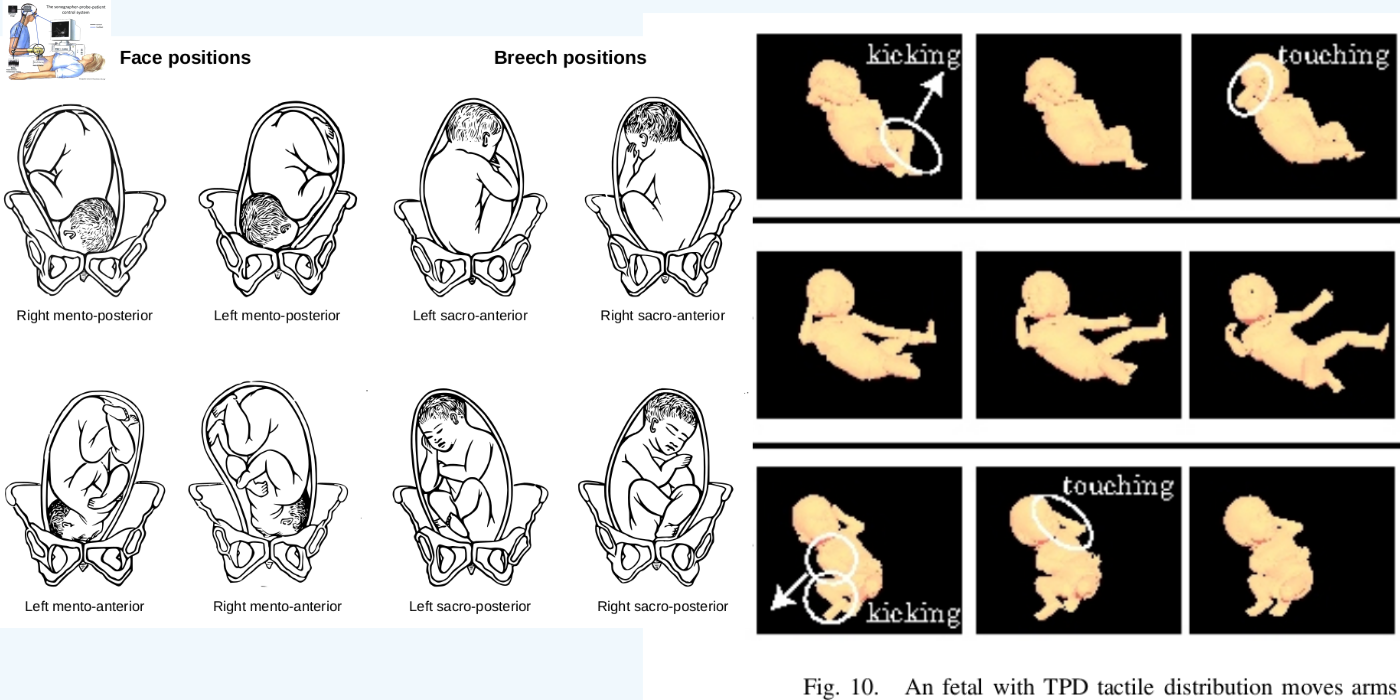
\includegraphics[width=1.0\textwidth]{one-slide-diagram/outputs/drawing-v00}
        % \caption{The sonographer-probe-patient control system}
      \end{figure}
\end{frame}
}



\end{document}
